%============%
\chapter{耳が縮む}
%============%
耳とは広辞苑によれば、
\\
  聴覚をつかさどる器官。人では外耳・中耳・内耳の3部に分かれ、外耳は耳介と外耳道とから成り、外耳道の内端には、空気の振動を伝える鼓膜がある。鼓膜の振動は、中耳にある3個の骨によって伝えられ内耳に達し、聴神経を刺激して聴覚を生じる。また、内耳には一般に平衡器官が含まれている。
\\
と定義されている。

\begin{figure}
  \centering
  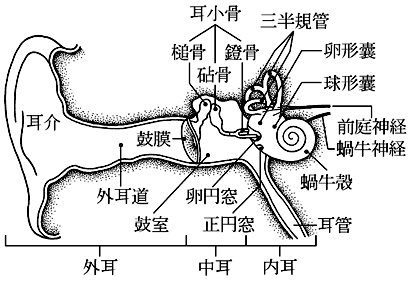
\includegraphics[scale=0.5]{./section/Mimi/figures/Koujien.jpg}
  \caption{耳の構造}
  \label{mimi}
\end{figure}

\par

本章では、本来は縮まないとされる耳が如何にして縮むのか、その最新研究結果を示す。
またその最新結果がいかにして発見されたかを、歴史的経緯から紐解こうと試みるのが本章の課題である。

%===================%
\section{歴史的経緯}
%===================%
以下では耳が縮んだ理由を歴史的事実を紐解くことにより、究明していこうと考える。
まずその大前提となるホワイトボードの導入を行い、次にそれらを使った行われていたディスカッションの方法を述べる。
そして本題である耳の縮む奇病について議論し、対策を論じ結論とする。

%---------------------------------%
\subsection{カワバタ式ホワイトボード}
%---------------------------------%
最初に我々が手に入れたホワイトボードという概念は、他称高槻市出身のカワバタ氏寄贈のホワイトボードである。
このホワイトボードは$50\rm{cm}\times30\rm{cm}$ほどの小ぶりのものであった。
そのため、このホワイトボードを誰がどのように使うかの議論が紛糾し、最終的にはジャンケンで勝った人間が、R2D2\footnote{小川ライフ店から無償提供される空き缶。}の頭を一つの単位とした
領地を取り合うという平和的解決策が採用されることとなった。

\begin{figure}
  \begin{center}
  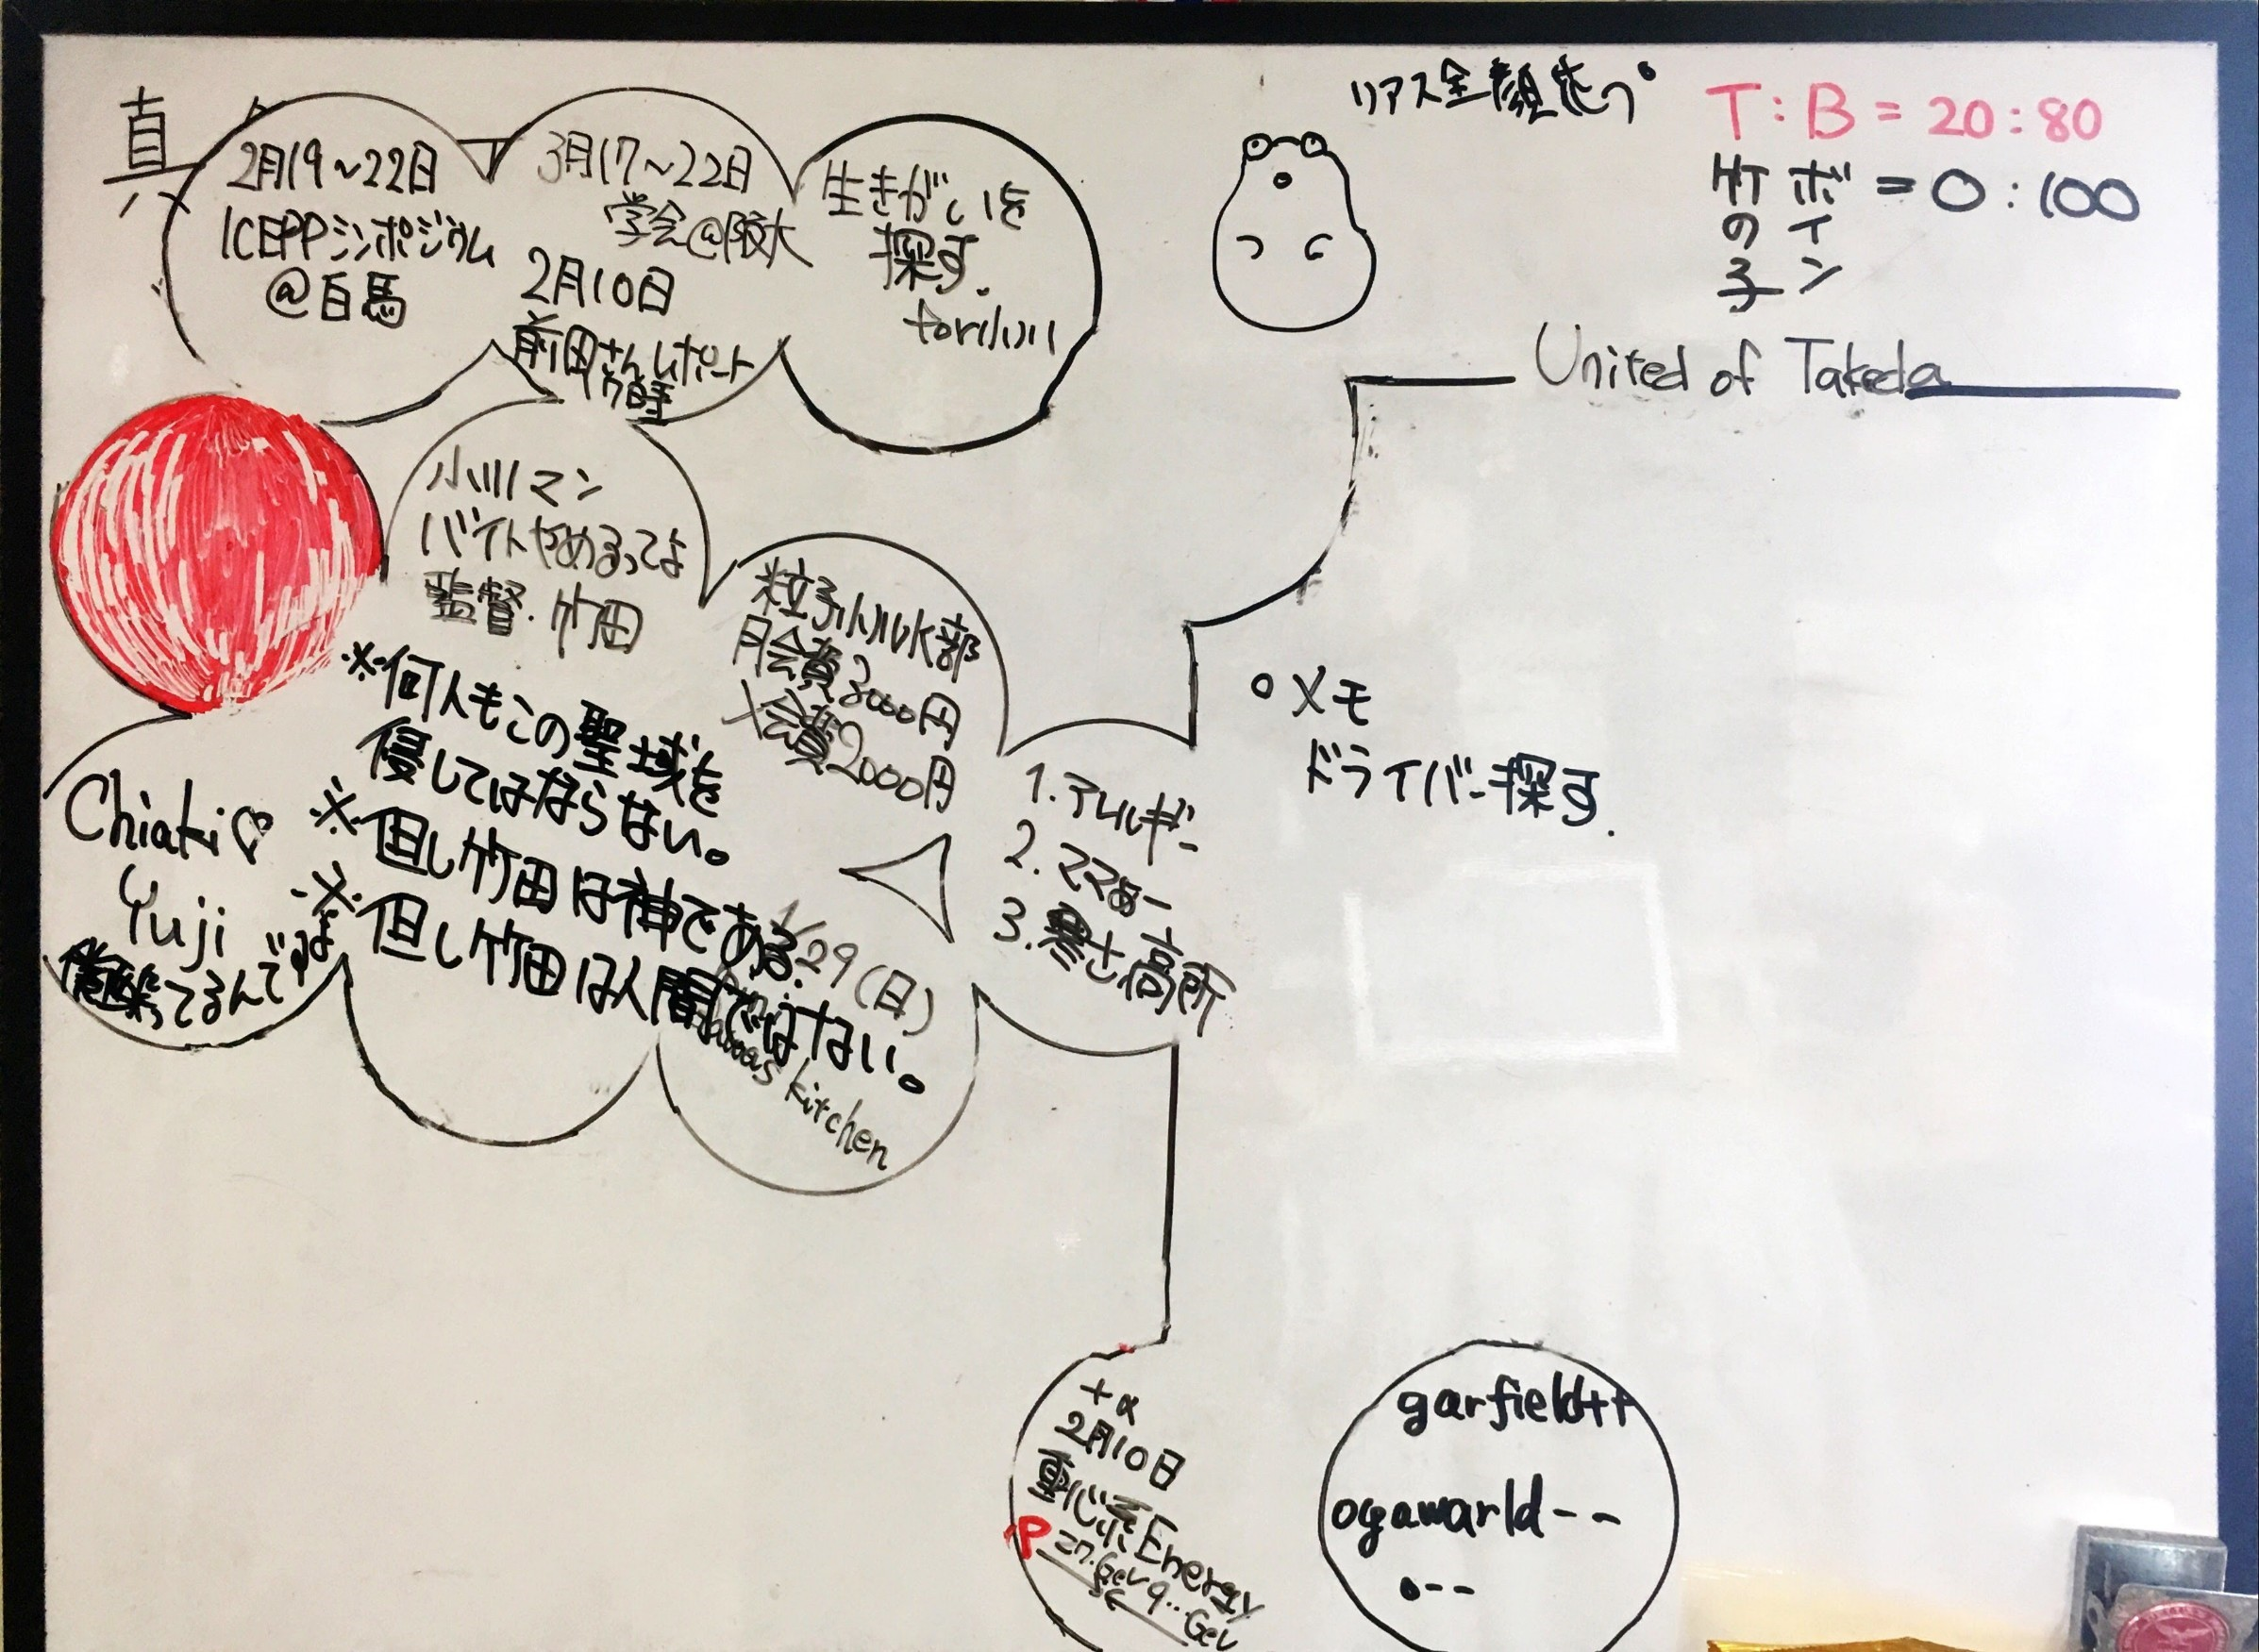
\includegraphics[width=0.6\textwidth]{./section/Mimi/figures/KawabataWhiteBoard.jpg}
    \caption{カワバタ式ホワイトボードの一例。竹田王国の領土が最大図版となっていた時代である。}
  \label{fig:KawabataWhiteBoard}
  \end{center}
\end{figure}

%--------------------------%
\subsection{壁ホワイトボード}
%--------------------------%
新しい学説が発表されたのは、2017年も年の瀬に近い12月後半である。
修士論文の締切の足音が近づいてきていたこの頃、竹田・オガワ・ミツタロウの三名は、ホワイトボードの前で喧々諤々と議論を繰り広げていた。
まず、以下ではホワイトボードに関する導入を行い、その後に爆誕した耳が縮む病気について議論し結論とする。
\par
我々は兼ねてから、議論を活発化するためにホワイトボードの必要性を感じていた。
小さなメモ程度のホワイトボードはオバツナ氏の寄贈により以前から存在していたものの、壁一面に自らのアイデアを記すことのできるほどの大きさをもつホワイトボードは設置されていなかった。
そこで、修士一年から二年に進級するときに、藏重教授に依頼し税金を投入しホワイトボードを設置していただくこととなった。
しかしどのような形式のホワイトボードを購入するかが次の問題となった。というのも、ホワイトボードを壁に設置したかったのであるが、設置したい壁が普通の壁(つまり金属でなくマグネット式の設置はできなかった)であったため、
裏面に接着剤の付いたホワイトボードの購入が決定された。
しかし、壁がざらついていたため、ホワイトボードの重さで接着剤が剥がれ落下してしまったのである。
さらなる不幸は続く。
もともと修士一年の際に購入して設置までしていたので、設置場所の壁近くに座っていたのは、その時点では我々ではなく、斎藤さんだぞ氏であった。
そのため管理がずさんであり、落下したホワイトボードを綺麗に保存することなく、部分的には折れ曲がるような形でオガワマンの机と返却されてくることになったのである
\footnote{以上からも分かるように、とりあえず斎藤さんだぞは無能なのである。また、オガワマンはキレたが、当然のことである。}。
そこでさらなる強力な接着剤の購入を依頼し、ようやくホワイトボードを設置することができたのである。
ホワイトボードには喧々諤々と、議論されたあとが見受けられる。

\begin{figure}
  \begin{center}
  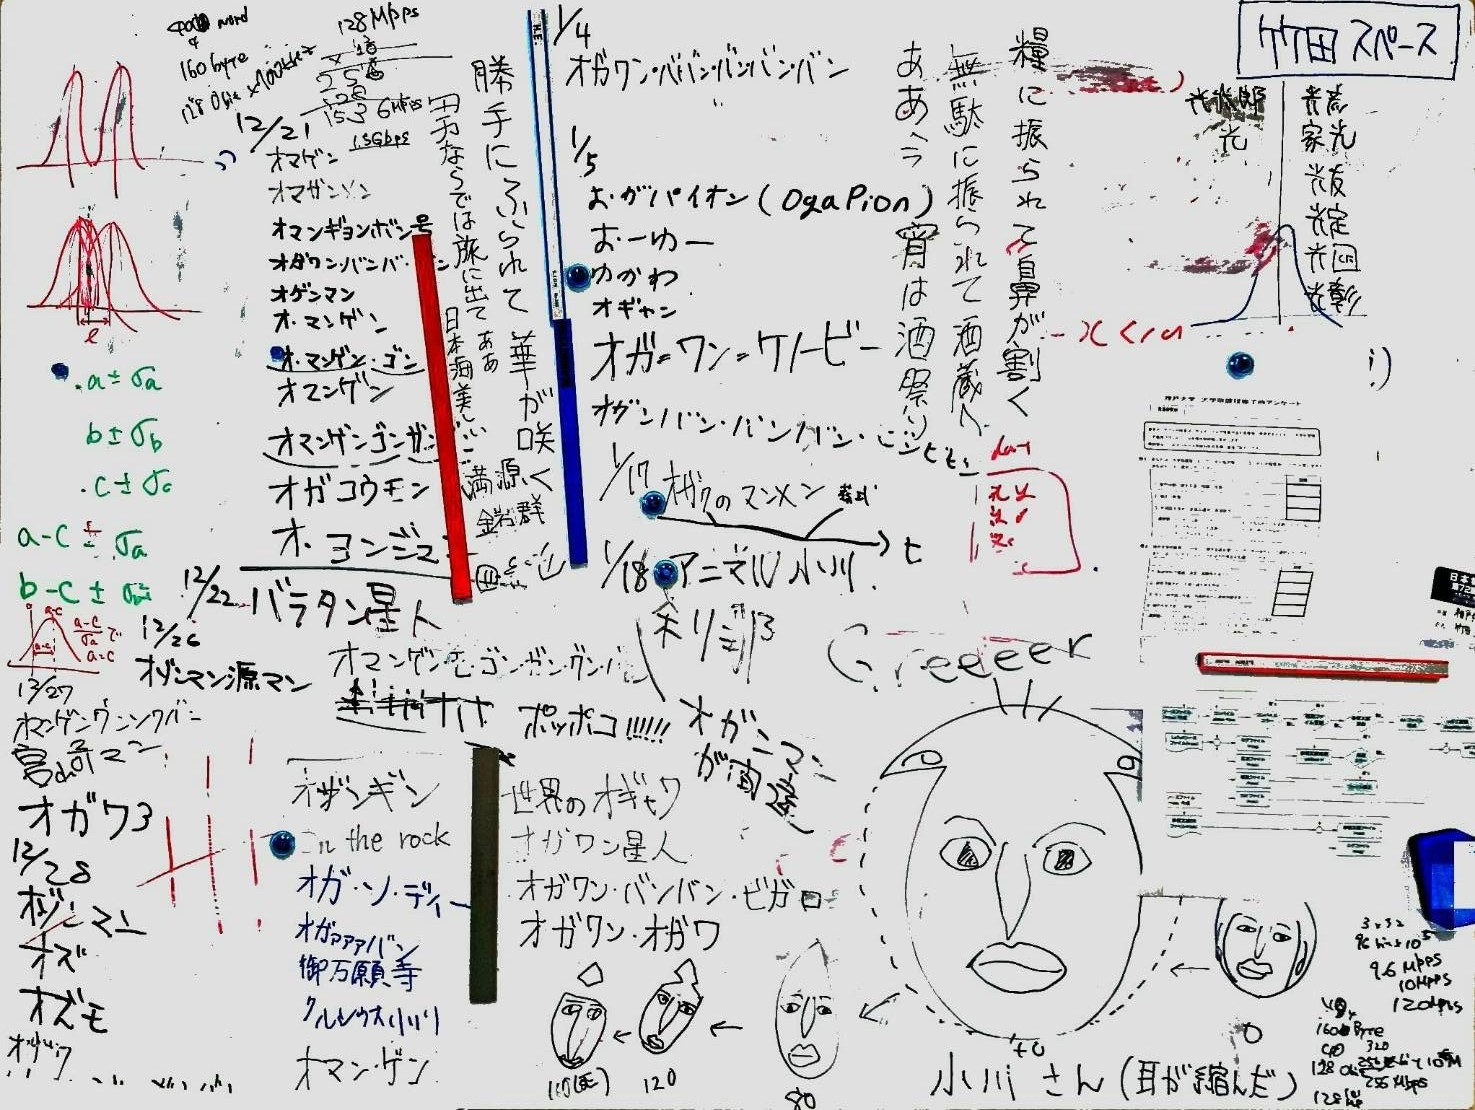
\includegraphics[width=0.6\textwidth]{./section/Mimi/figures/WhiteBoard.jpg}
  \caption{ホワイトボードの一例。この時点のホワイトボードには、2017年12月21日から2018年1月18日の小川圭将のニックネームが記されている。
    また右上には、「光という漢字を"コウ"と読むのは稀有であるので、若宮光太郎は、ミツタロウと呼ぶのが正しい」という議論が繰り広げられた痕跡が残されている。
    この時点のホワイトボードを見るに、光を"ミツ"と呼ぶケースが大多数挙げられている。}
  \label{fig;WhiteBoard}
  \end{center}
\end{figure}

ホワイトボードによる議論は非常に活発に行われ、特に修士論文の締切が近づいてきたときには、まずアイデアをホワイトボードに書き起こし、
それらを元にとにかく解析を進めるという作業スタイルが確立され、非常に効率の良い研究が進められたとオガワマンは語っている(図\ref{fig:OgawaChidori})。

\begin{figure}
  \begin{center}
  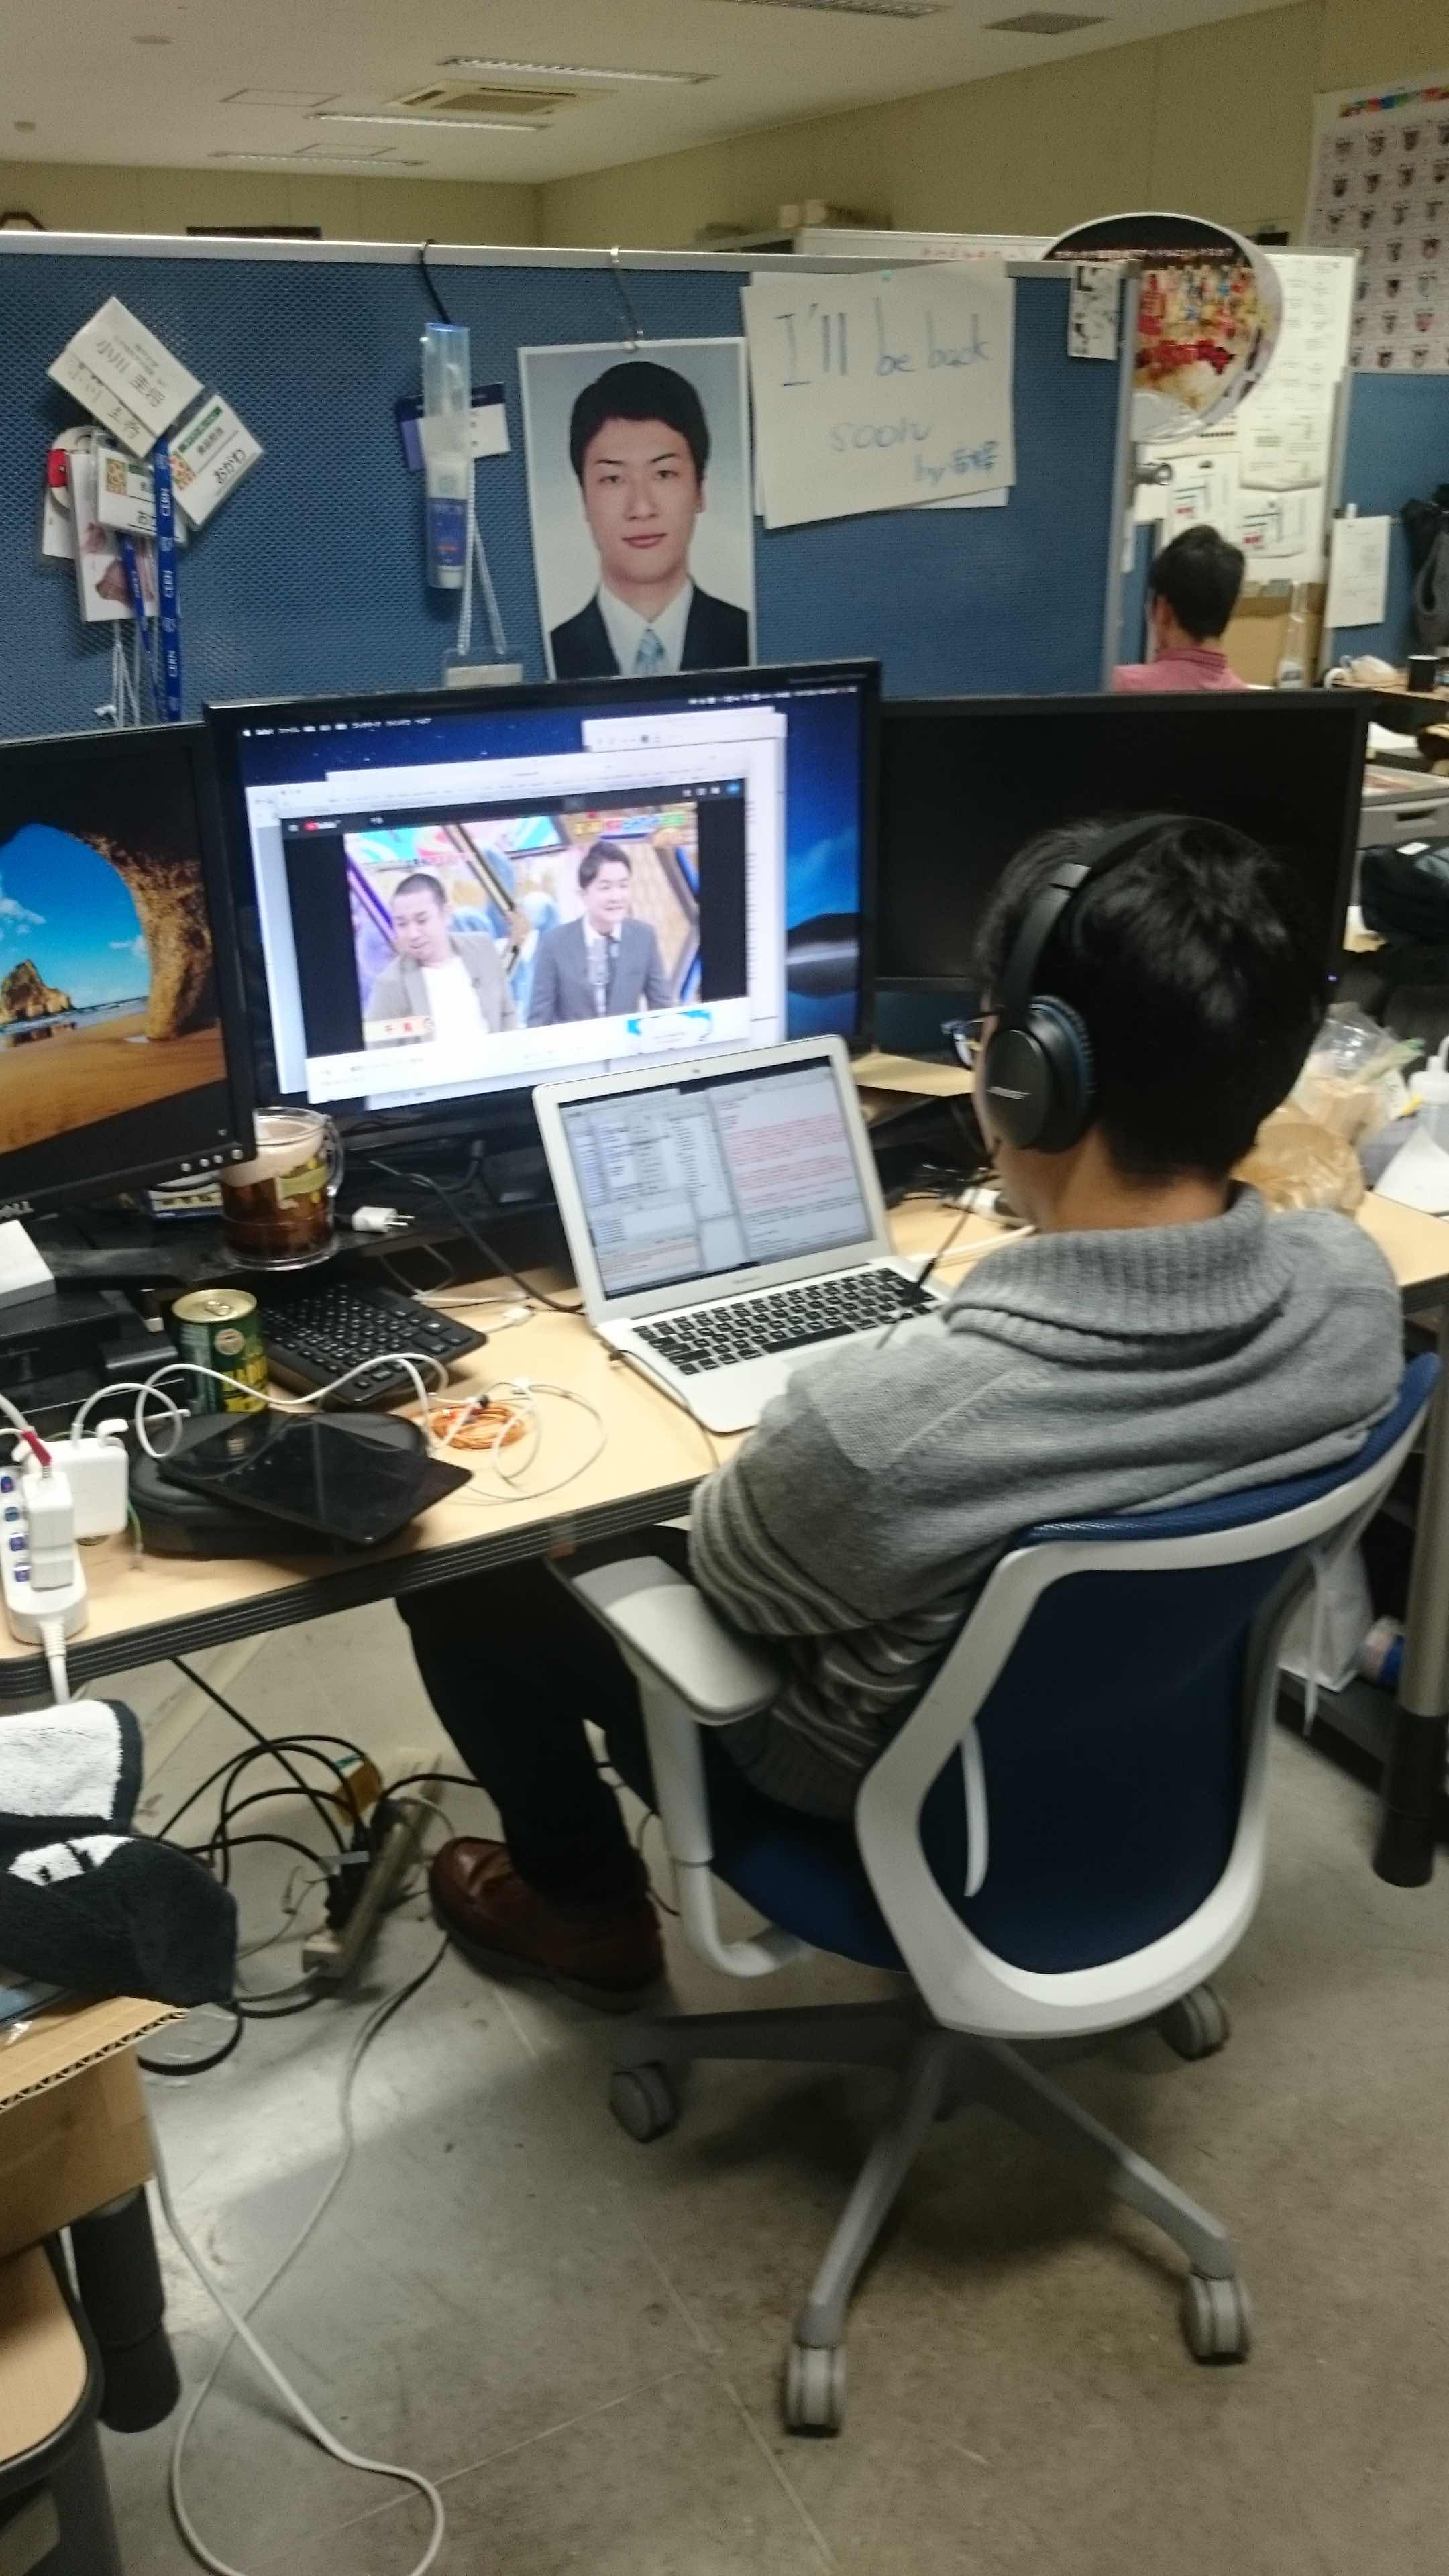
\includegraphics[width=0.4\textwidth]{./section/Mimi/figures/OgawaChidori.jpg}
  \caption{ホワイトボードによる議論を元に研究に取り組む一例。本研究者のディスプレイを観察すると、どうやら千鳥の漫才を研究している様である。
    また、ディスプレイの上には自らの証明写真を拡大した写真が飾られており、後ろにも目がありお前たちの行動も観察しているぞ、との意志の表れであろうか。}
  \label{fig:OgawaChidori}
  \end{center}
\end{figure}

%--------------------------------------%
\subsection{年末帰省時の変なテンション}
%--------------------------------------%
以上まででホワイトボードについて簡単に説明が済んだことと思う。
そこで本題に移る。
\par
時期は、先に述べたように年末の帰省のタイミングである。
このタイミングで我々は、ホワイトボードの前に集まり集会を開いていた。
議題はオガワカヲリである(\ref{chap:Kawori}章参照)。

%--------------------------------------%
\section{一般的な耳縮の主な原因}
%--------------------------------------%
耳の素材により異なるが、そもそもなぜ耳は縮むのかという一般的な問題提起から論じる。
特に本研究では注意すべき耳の素材のひとつ「綿」についての提起となる。
耳がどのように初期の受精卵から形成されていくかについてまず簡単に説明する。
まず、綿(コットン)が耳になるまでには、原綿(コットンボール) を繊維が揃う状態になるまで引き揃え、そこから耳になるよう、受精卵を持った母体が責任を持って作成していく。
この紡ぐ工程の際に繊維を引っ張りながら撚りをかけていくのだが、引っ張られた繊維は元に戻ろうとする力が働き、これが耳の縮みの主な原因のひとつとなる。
そうしたことから一般的な病院では耳を作る過程で、耳を叩き縮みやゆがみを軽減させる工程を踏む。\par

そうすることで、作る耳にゆがみやムラがなく、均一に仕上げることが出来る。
ただこうした工程を踏まえても完全に縮まないというわけではない。
さらに、耳は水を含むと膨張します。
その状態で、ドライヤーなどで乾かすと膨張した耳が急激に元に戻ろうとし、
その結果、耳が縮むという現象が起こる。

%--------------------------------------%
\section{本研究の対象となる事象}
%--------------------------------------%
本研究では、若宮非言語大学特任学長が発見した図\ref{mimi}に示す、耳縮カオリ過程(ワカミヤ・カオリ過程)についての研究となる。
\begin{figure}
\centering
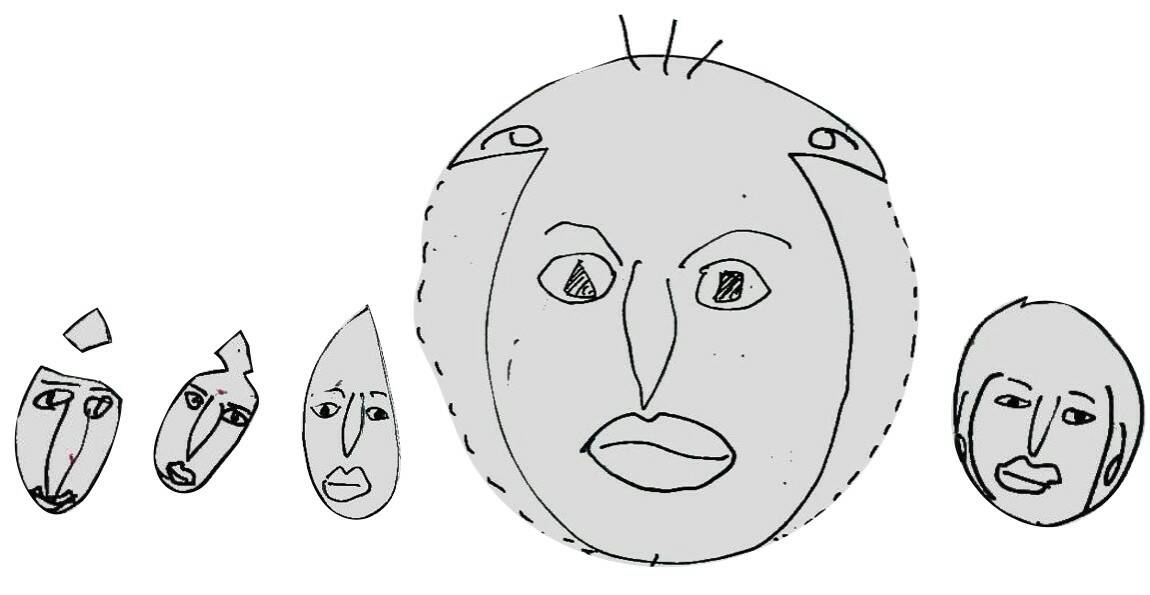
\includegraphics[scale=0.3]{mimi.jpg}
\caption{耳の縮む過程}
\label{mimi}
\end{figure}
この過程では、右から左に時間軸を取りどの様に耳が縮んでいくかの化学式を示している。
最も大きく強調されている化学式には破線を用い補助的な線を引いている。
このワカミヤ・カオリ過程によれば、生まれた時耳は顔にへばりついているのだが、年を取るに従い、前述の一般的な原因に従い耳が縮んでいき、最終的に耳が取れる。
取れた耳は、種子として次世代の耳へと受け継がれていく。
